\documentclass[10pt]{beamer}
\usetheme{Warsaw}

\usepackage[polish]{babel}
\usepackage[utf8]{inputenc}
\usepackage[T1]{fontenc}


\usepackage{latexsym,gensymb,amsmath,amssymb,amsthm}
\usepackage{graphicx}
\usepackage{url}

\usepackage{graphics}






\usepackage{hyperref}

\usepackage{algorithmicx}
\usepackage{algorithm}
\usepackage{graphicx}
\usepackage{epstopdf}
\usepackage{algpseudocode}
\usepackage{float}

\title[Flow Shop Scheduling Problem]{Flow~Shop~Scheduling~Problem}
\author[Krzysztof Chrobak\and Jan Sochiera]{Krzysztof~Chrobak \and Jan~Sochiera}
	

\institute[Algorytmy Ewolucyjne 2012]{\normalsize Algorytmy Ewolucyjne 2012}
\subject{Computational Sciences}


\begin{document}

\frame{
\titlepage
}


\section{Definicja problemu}
\frame{
  \frametitle{Definicja problemu}

  \begin{itemize}
    \item<1-> $n$ zadań
    \item<2-> $m$ maszyn
    \item<3-> Każde zadanie musi być wykonane na każdej maszynie
    \item<4-> Każda maszyna musi wykonaywać zadania w tej samej kolejności
    \item<5-> Jedno zadanie nie może być wykonywane jednocześnie na więcej niż jednej maszynie
  \end{itemize}
}


\section{Przestrzeń przeszukiwania}
\frame
{
  \frametitle{Histogram}
	\begin{figure}
\begin{center}
%  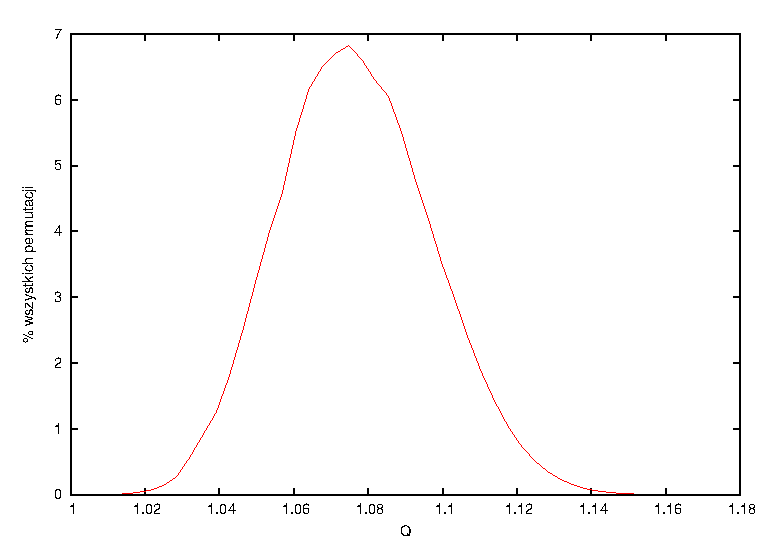
\includegraphics{histogram.eps}
\end{center}
\end{figure}
}


\frame
{
  \frametitle{Dystrybuanta}
\begin{figure}
\begin{center}
%  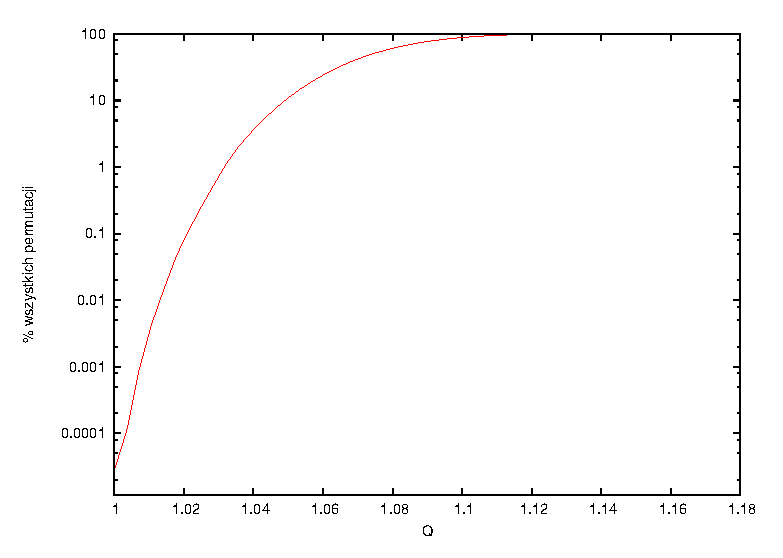
\includegraphics{dystrybuanta.eps}
\end{center}
\end{figure}

	
}

\section{Algorytm}
\frame
{
  \frametitle{Algorytm}
  Algorytm który zaimplementowaliśmy jest modyfikacją klasycznego SGA, do której dodaliśmy przeszukiwanie lokalne
i zwiększanie różnorodności populacji poprzez dodawanie losowych imigrantów. Dane wejściowe dla tego algorytmu:
\begin{description}
  \item[instance] instancja problemu flow shop
  \item[population\_size] rozmiar populacji
  \item[num\_parents] ilość rodziców
  \item[mutation\_probability] prawdopodobieństwo mutacji
  \item[$\alpha$] parametr imigracji
  
\end{description}

}

\frame
{
  \frametitle{Algorytm}

\begin{algorithm}[H]
\caption{Algorytm ewolucyjny dla problemu flow shop}
\label{algorytm}
\begin{algorithmic}
  \State $P \gets RandomPopulation(population\_size)$
  \State $EvaluatePopulation(P, instance)$
  \While{not $TerminationCondition(P)$}
    \State $Parents \gets SelectParents(P, num\_parents)$ 
    \State $Children \gets Crossover(Parents)$
    \State $Children \gets Mutate(Children, mutation\_probability)$
    \State $Children \gets LocalSearch(Children, instance)$
    \State $Population \gets Replace(Population, Children)$
    \State $Population \gets AddImigrants(Population, instance, \alpha)$
  \EndWhile
\end{algorithmic}
\end{algorithm}
}

\frame
{
\frametitle{Ocena osobników $EvaluatePopulation$}

 Pojedynczego osobnika można ocenić przy pomocy prostego algorytmu dynamicznego, korzystającego
z następujących zależności ($E[i,j]$ to czas zakończenia wykonywania $j$-tego w kolejności zadania
na $i$-tej maszynie, przy kolejności zadań $\pi$):
$$ E[1, 1] = t_{1,\pi(1)} $$
$$ E[1, i] = E[1, i-1] + t_{1,\pi(i)}\ \  i = 2 \ldots n$$
$$ E[i, 1] = E[i-1, 1] + t_{i,\pi(1)}\ \  i = 2 \ldots m$$
$$ E[i, j] = max(E[i-1, j], E[i, j-1]) + t_{i, \pi(j)} \ \ i = 2 \ldots n \ \ j = 2 \ldots m $$
Algorytm dynamiczny oceny jednego osobnika ma złożoność $O(nm)$

}

\frame
{
\frametitle{Warunek zakończenia $TerminationCondition$}
Nasz algorytm kończy działanie gdy przekroczy ustaloną z góry ilość iteracji pętli while, albo
gdy uda mu się osiągnąć wartość funkcji celu znaną jako optymalna dla danego problemu. Oczywiście
ten ostatni warunek należałoby usunąć chcąc rozwiązywać nowe problemy, ale podczas testowania 
algorytmu szukanie rozwiązania lepszego niż optymalne nie miało żadnego sensu.

}

\frame
{
\frametitle{Wybór rodziców $SelectParents$}
Eksperymentowaliśmy z dwiema metodami wyboru rodziców:
\begin{itemize}
  \item Metoda ruletki z różnymi skalowaniami funkcji przystosowania
  \item Metoda k-najlepszych osobników
\end{itemize}
W ostatecznej wersji algorytmu zdecydowaliśmy się na drugą metodę, ponieważ
w połączeniu z metodą ruletki nie dało się stosować wybranej przez nas strategii zastępowania. Okazało 
się również, że warto pozwalać wszystkim osobnikom wziąć udział w reprodukcji.
}

\frame
{
\frametitle{Krzyżowanie $Crossover$}
Osobniki wybrane do reprodukcji są losowo kojarzone w pary, tak że każdy ma dokładnie jednego partnera.
Do krzyżowania użyliśmy prostego operatora PMX.
}

\frame
{
\frametitle{Mutacja $Mutate$}
Z pewnym małym prawdopodobieństwem (po kilku eksperymentach ustaliliśmy tą wartość na 5\%) każde dziecko jest
mutowane. Mutacja polega na złożeniu permutacji osobnika z losową permutacją o około 75\% punktów stałych.
}


\frame
{
\frametitle{Przeszukiwanie lokalne $LocalSearch$}

\begin{algorithm}[H]
\caption{Przeszukiwanie lokalne}
\label{localsearch}
\begin{algorithmic}
  \For {$i \gets 1 \ldots |Children|$}
    \State $I \gets Children[i]$
    \State $best \gets I$
    \State $mspan \gets makespan(I)$
    \For {$j \gets 1 \ldots n$}
      \For {$k \gets 1 \ldots n$}
        \State $Candidate \gets insert(I, i, k)$
        \State $cspan \gets makespan(Candidate)$
        \If{$cspan < mspan $}
          \State $mspan \gets cspan$
          \State $best \gets Candidate$
        \EndIf
      \EndFor
    \EndFor
    \State $Children[i] = best$
  \EndFor
\end{algorithmic}
\end{algorithm}

}



\frame
{
\frametitle{Zastępowanie $Replace$}
Aby uniemożliwić najlepszym osobnikom zdominowanie populacji po kilku iteracjach, użyliśmy schematu
zastępowania, który bierze pod uwagę tylko czwórkę osobników : parę rodziców i ich dzieci. Z takiej
czwórki wybieramy 2 najlepszych osobników, i to oni przechodzą do następnego pokolenia. Oczywiście
tą procedurę należy powtórzyć dla wszystkich par rodziców wygenerowanych w kroku krzyżowania.


}



\frame
{
\frametitle{Imigracja $AddImigrants$}
Aby algorytm działał dowolnie długo, postanowiliśmy mierzyć różnorodność osobników w populacji i w razie jej
spadku zastępować najgorsze osobniki losowymi. Wprowadziliśmy współczynnik różnorodności $D$:
$$ D = \frac{\text{ilość różnych osobników}}{\text{ilość osobników}} $$
Ilość osobników zastępowanych losowymi jest określona przez parametr $\alpha$ i zależność:
$$ N_{random} = \lfloor \alpha * (1 - D) * population\_size  \rfloor $$
Aby nowe osobniki nie zostały wyeliminowane po jednej iteracji, wykonujemy dla każdego z nich przeszukiwanie
lokalne.



}



\frame
{
\frametitle{Implementacja}
Algorytm zaimplementowaliśmy w C++ przy użyciu biblioteki OpenMP, która umożliwiła nam łatwe zrównoleglenie
przeszukiwania lokalnego (ten proces jest niezależny dla każdego osobnika).

}

\section{Wyniki}

\frame
{

\frametitle{Parametry algorytmu}

\begin{table}[H]
\caption{Wartości parametrów algorytmu}
\label{parametry}
\begin{center}
\begin{tabular}{|l|l|}
  \hline
  parametr & wartość \\
  \hline
  rozmiar populacji & 1000 \\
  ilość rodziców & 1000 \\
  prawdopodobieństwo mutacji & 0.05 \\
  $\alpha$ & 0.3 \\
  \hline
\end{tabular}
\end{center}
\end{table}

}



\frame
{
\begin{table}[H]
\caption{Najlepsze znalezione rozwiązanie}
\label{best}
\begin{center}
\begin{tabular}{|l|l|l|l||l|l||l|l|}
  \hline
  $n$ & $m$ & $id$ & $opt$ & $opt_{ev}$ & $opt_{random}$ & $Q_{ev}$ & $Q_{random}$ \\
  \hline
  20 & 5 & 0 & 1278 & 1278 & 1296 & 1.0 & 1.014 \\
  20 & 10 & 0 & 1582 & 1582 & 1657 & 1.0 & 1.047 \\
  20 & 20 & 0 & 2297 & 2297 & 2381 & 1.0 & 1.036 \\
  50 & 5 & 0 & 2724 & 2724 & 2744 & 1.0 & 1.007 \\
  50 & 10 & 0 & 3025 & 3025 & 3293 & 1.0 & 1.088 \\
  50 & 20 & 0 & 3875 & 3893 & 4315 & 1.004 & 1.113 \\
  100 & 10 & 0 & 5770 & 5770 & 6242 & 1.0 & 1.081 \\
  100 & 20 & 0 & 6286 & 6304 & 7112 & 1.002 & 1.131 \\
  200 & 10 & 0 & 10868 & 10872 & 11403 & 1.001 & 1.049 \\
  500 & 20 & 0 & 26189 & 26249 & 28806 & 1.002 & 1.099 \\
  500 & 20 & 1 & 26629 & 26700 & 29169 & 1.002 & 1.095 \\
  \hline
\end{tabular}
\end{center}
\end{table}


}

\frame{

\begin{table}[H]
\caption{Średnie najlepsze znalezione rozwiązanie}
\label{mean}
\begin{center}
\begin{tabular}{|l|l|l|l||l|l||l|l|}
  \hline
  $n$ & $m$ & $id$ & $\overline{opt_{ev}}$ & $\overline{opt_{random}}$ & $Dopt_{ev}$ & $Dopt_{random}$ \\
  \hline
  20 & 5 & 0 & 1278.0 & 1296.8 & 0.0 & 0.314 \\
  20 & 10 & 0 & 1582.4 & 1675.6 & 0.942809041582 & 8.53 \\
  20 & 20 & 0 & 2297.4 & 2407.2 & 0.666 & 13.219 \\
  50 & 5 & 0 & 2724.0 & 2753.4 & 0.0 & 5.209 \\
  50 & 10 & 0 & 3036.8 & 3342.2 & 4.565 & 19.048 \\
  50 & 20 & 0 & 3896.4 & 4342.8 & 3.8 & 13.464 \\
  100 & 10 & 0 & 5776.0 & 6264.6 & 6.236 & 14.605 \\
  100 & 20 & 0 & 6319.4 & 7143.6 & 11.275 & 18.499 \\
  200 & 10 & 0 & 10876.4 & 11436.8 & 6.128 & 16.251 \\
  500 & 20 & 0 & 26284.6 & 28858.4 & 15.114 & 29.295 \\
  500 & 20 & 1 & 26738.2 & 29266.2 & 21.183 & 47.115 \\
  \hline
\end{tabular}
\end{center}
\end{table}

}


\frame{


\frametitle{Działanie algorytmu}
W każdej iteracji algorytmu zapisywaliśmy średnią wartość funkcji $makespan$ dla całej populacji
oraz dla najlepszego osobnika. Wykres progress przedstawia jak zmieniają się te wartości 
podczas jednego uruchomienia algorytmu dla trudnego problemu ($m = 20$, $n = 500$). Widać na nim
że mimo że postęp jest coraz wolniejszy, to algorytm nie pozwala by średnia wartość stała się równa
najlepszej, tym samym zabezpieczając populację przed staniem się zbiorem kopii jednego osobnika.

Wykres diversity przedstawia wartość współczynnika różnorodności w zależności od numeru iteracji.
Widać na nim, że algorytm stara się utrzymać możliwie wysoką wartość tego wskaźnika, lecz z czasem
wylosowanie osobnika, który różnił by się od wszystkich istniejących i jednocześnie miał na tyle
dobrą wartość funkcji $makespan$, by przetrwać proces selekcji jest coraz trudniejsze.
}

\section{Wnioski}  

\frame{
\frametitle{Zbieżność algorytmu}
Wykresy progress, diversity pokazują, że o ile jakość znalezionego rozwiązania z czasem polepsza się 
coraz wolniej, to różnorodność populacji jest utrzymywana na wysokim poziomie. Oznacza to, że nasz algorytm jest odporny na utykanie
w minimach lokalnych, i nie przestanie działać z powodu zdominowania populacji przez jednego osobnika. Jest to
zasługa strategii zastępowania i losowej imigracji, które chronią różnorodność populacji.
}

\frame{
\frametitle{Ograniczenia na wielkość problemu}
{\huge Pamięciowe}\\
W wypadku naszego algorytmu ograniczeniem jest wyłącznie czas jego działania, ponieważ
pamięć zużywana na przechowywanie populacji jest niezmienna w czasie i proporcjonalna do
$n \cdot population\_size$, co nie stanowi żadnego problemu dla współczesnych komputerów.
{\huge Czasowe}\\
Złożoność pojedynczej iteracji jest zdominowana przez czas przeszukiwania lokalnego, który wynosi
$O(mn^2|Children|)$, zatem złożoność całego algorytmu to $O(smn^2|Children|)$, gdzie $s$ to ilość iteracji.
Trudno powiedzieć, jaka jest górna granica rozmiaru rozwiązywalnego problemu, ponieważ przeszukiwanie 
lokalne jest zaimplementowane równolegle, czyli stała ukryta w notacji $O$ jest odwrotnie proporcjonalna
do liczby procesorów komputera na którym uruchamiamy algorytm. 
}

\frame{

\begin{table}[H]
\caption{Średni czas iteracji dla 1000 osobników}
\label{sredniaiteracja}
\begin{center}
\begin{tabular}{|l|l|l|}
  \hline
  n & m & średni czas iteracji \\
  \hline
  500 & 20 & 7.3 s \\
  200 & 20 & 1.27 s \\
  200 & 10 & 0.72 s \\
  100 & 20 & 0.36 s \\
  100 & 10 & 0.18 s \\
  100 & 5 & 0.09 s \\
  \hline
\end{tabular}
\end{center}
\end{table}

}


\end{document}
